\title{Update: Agent consensus via sources of opportunity}

\date{\today}

\documentclass[12pt]{article}

\usepackage{amssymb}
\usepackage{graphicx}
\usepackage{float}

\begin{document}
\maketitle

\begin{abstract}
	Simulated some of the results from W. Ren paper from 2004. Use of row stochastic matrices and an uncommon matrix-graph representation to determine when spanning trees occur in dynamically changing weighted directed graphs. The spanning tree condition is necessary and sufficient to determine if information from communicating agents will converge. Successful simulation results presented for discrete-time dynamics case. 
\end{abstract}

\section{Introduction}
In consensus problems there are, in general, two popular goals people hope to achieve: 1) "average consensus" -- where the contribution from each agent (in the information convergence) is equal, and 2) "consensus" -- where there is (simply, not necessarily average) agreement. In case 1) the final value is equally weighted based on the initial conditions of each agent. This is a stronger condition than in 2) where in the second case the final consensus is dependent on additional parameters. \\

In consensus problems (cases 1 and 2) a common approach is to utilize algebraic graph theory concepts, usually something to do with the Laplacian, to determine what topological properties (if any!) a graph is required to have in order to achieve some form of consensus between information distributed among its vertices. This is studied from the perspective of both static and dynamically changing graph topologies. \\

In [1] he presents a technique where he (instead!) utilizes stochastic matrices to determine that convergence of information on a graph occurs iff there exists a spanning tree in the union of graphs over a finite (time/step) horizon. I will briefly detail this idea below. \\

Let $\mathcal{A} = \{A_{i} | i \leq n \in \mathcal{I} \}$ be a set of $n$ agents indexed on $\mathcal{I}$. A directed graph, $\mathcal{G}$, can be used to model the communication interations between these agents, where a directed edge from $A_{i}$ to $A_{j}$ can be represented as $(A_{i}, A_{j})$. Additionally, the topology of the directed graph can change dynamically with $\bar{\mathcal{G}} = \{ \mathcal{G}_{1}, \mathcal{G}_{2}, ... \mathcal{G}_{M} \}$ representing the union of these graphs. \\

I will now define the two required graph representations and the discrete-time dynamics defining the agent interactions. The dynamics are given as:

\begin{equation}
	\xi_{i}[k+1] = \frac{1}{\sum_{j=1}^{n} \alpha_{ij}[k]G_{ij}[k]} \sum_{j=1}^{n} \alpha_{ij}[k]G_{ij}[k]\xi_{j}[k]
\end{equation}

Where $\alpha_{ij} > 0$ is a weighing factor (allows for weighted directed graphs), $G_{ii}[k] \triangleq 1$, and $G_{ij}[k]$ is 1 if there is information floring from $A_{j}$ to $A_{i}$ at $t= kT$ (the discrete step). This can otherwise be written as in a lumped-parameter way as:

\begin{equation}
	\xi_{i}[k+1] = D[k]\xi[k]
\end{equation}

Note that we now have two distinct matrices, $G$ and $D$, where $G$ has 1s on the diagonal (a bit un-convential) and is otherwise an adjacency matrix and $D$ is what is called a "row stochastic matrix". This simply means that the rows all sum to 1, a form of normalization. It is shown in [1] that a spanning tree in the union of graphs is sufficient and necessary to achieve convergence in $\xi[k]$. This means there is a simply a directed tree in the graph that connects all vertices. A spanning tree is present iff $G$ with a negated diagonal (-1) has exactly 1 zero-eigenvalue. One last note is that $D$ is an "SIA" matrix (stochastic, indecomposable, and aperiodic), and if there exists a spanning tree in modified $G$ then $D_{m} ... D_{2}D_{1}$ converges over $m$ time/communication steps. \\

I check the rank of modified $G$, noting when a spanning tree is present in the union of $G_{i}$, then resetting the union calculation. This process also yields stochastic matrices $D_{i}$ that multiply one another from the left. The updated $D$ matrix at each step $k$ is multipled against $\xi[k]$. Simulation results are shown below.

\section{Results}\label{results}

I randomly initialized 4 agents inside an axis-aligned square boundary (10x10; 20x20; and 30x30 shown) using a uniform distribution. Each step the agents would be completely reinitialized. An edge in the graph $G$ between agents would be created if the distance between them was inside a ball of radius $2.0$; a new graph was generated and logged each step. The union of these graphs (simple, un-weighted; 0 or 1) was analyzed to check for a spanning tree, this is noted as a vertical line in the plots. \\

The plots show below are 04 randomly selected results from the 1000 run simulation, but all results converged. Note the difference in the number of communication steps required for convergence as the boundaries change, as well as how many steps it takes for each spanning tree to be realized (before being reset).

\begin{figure}[H]
	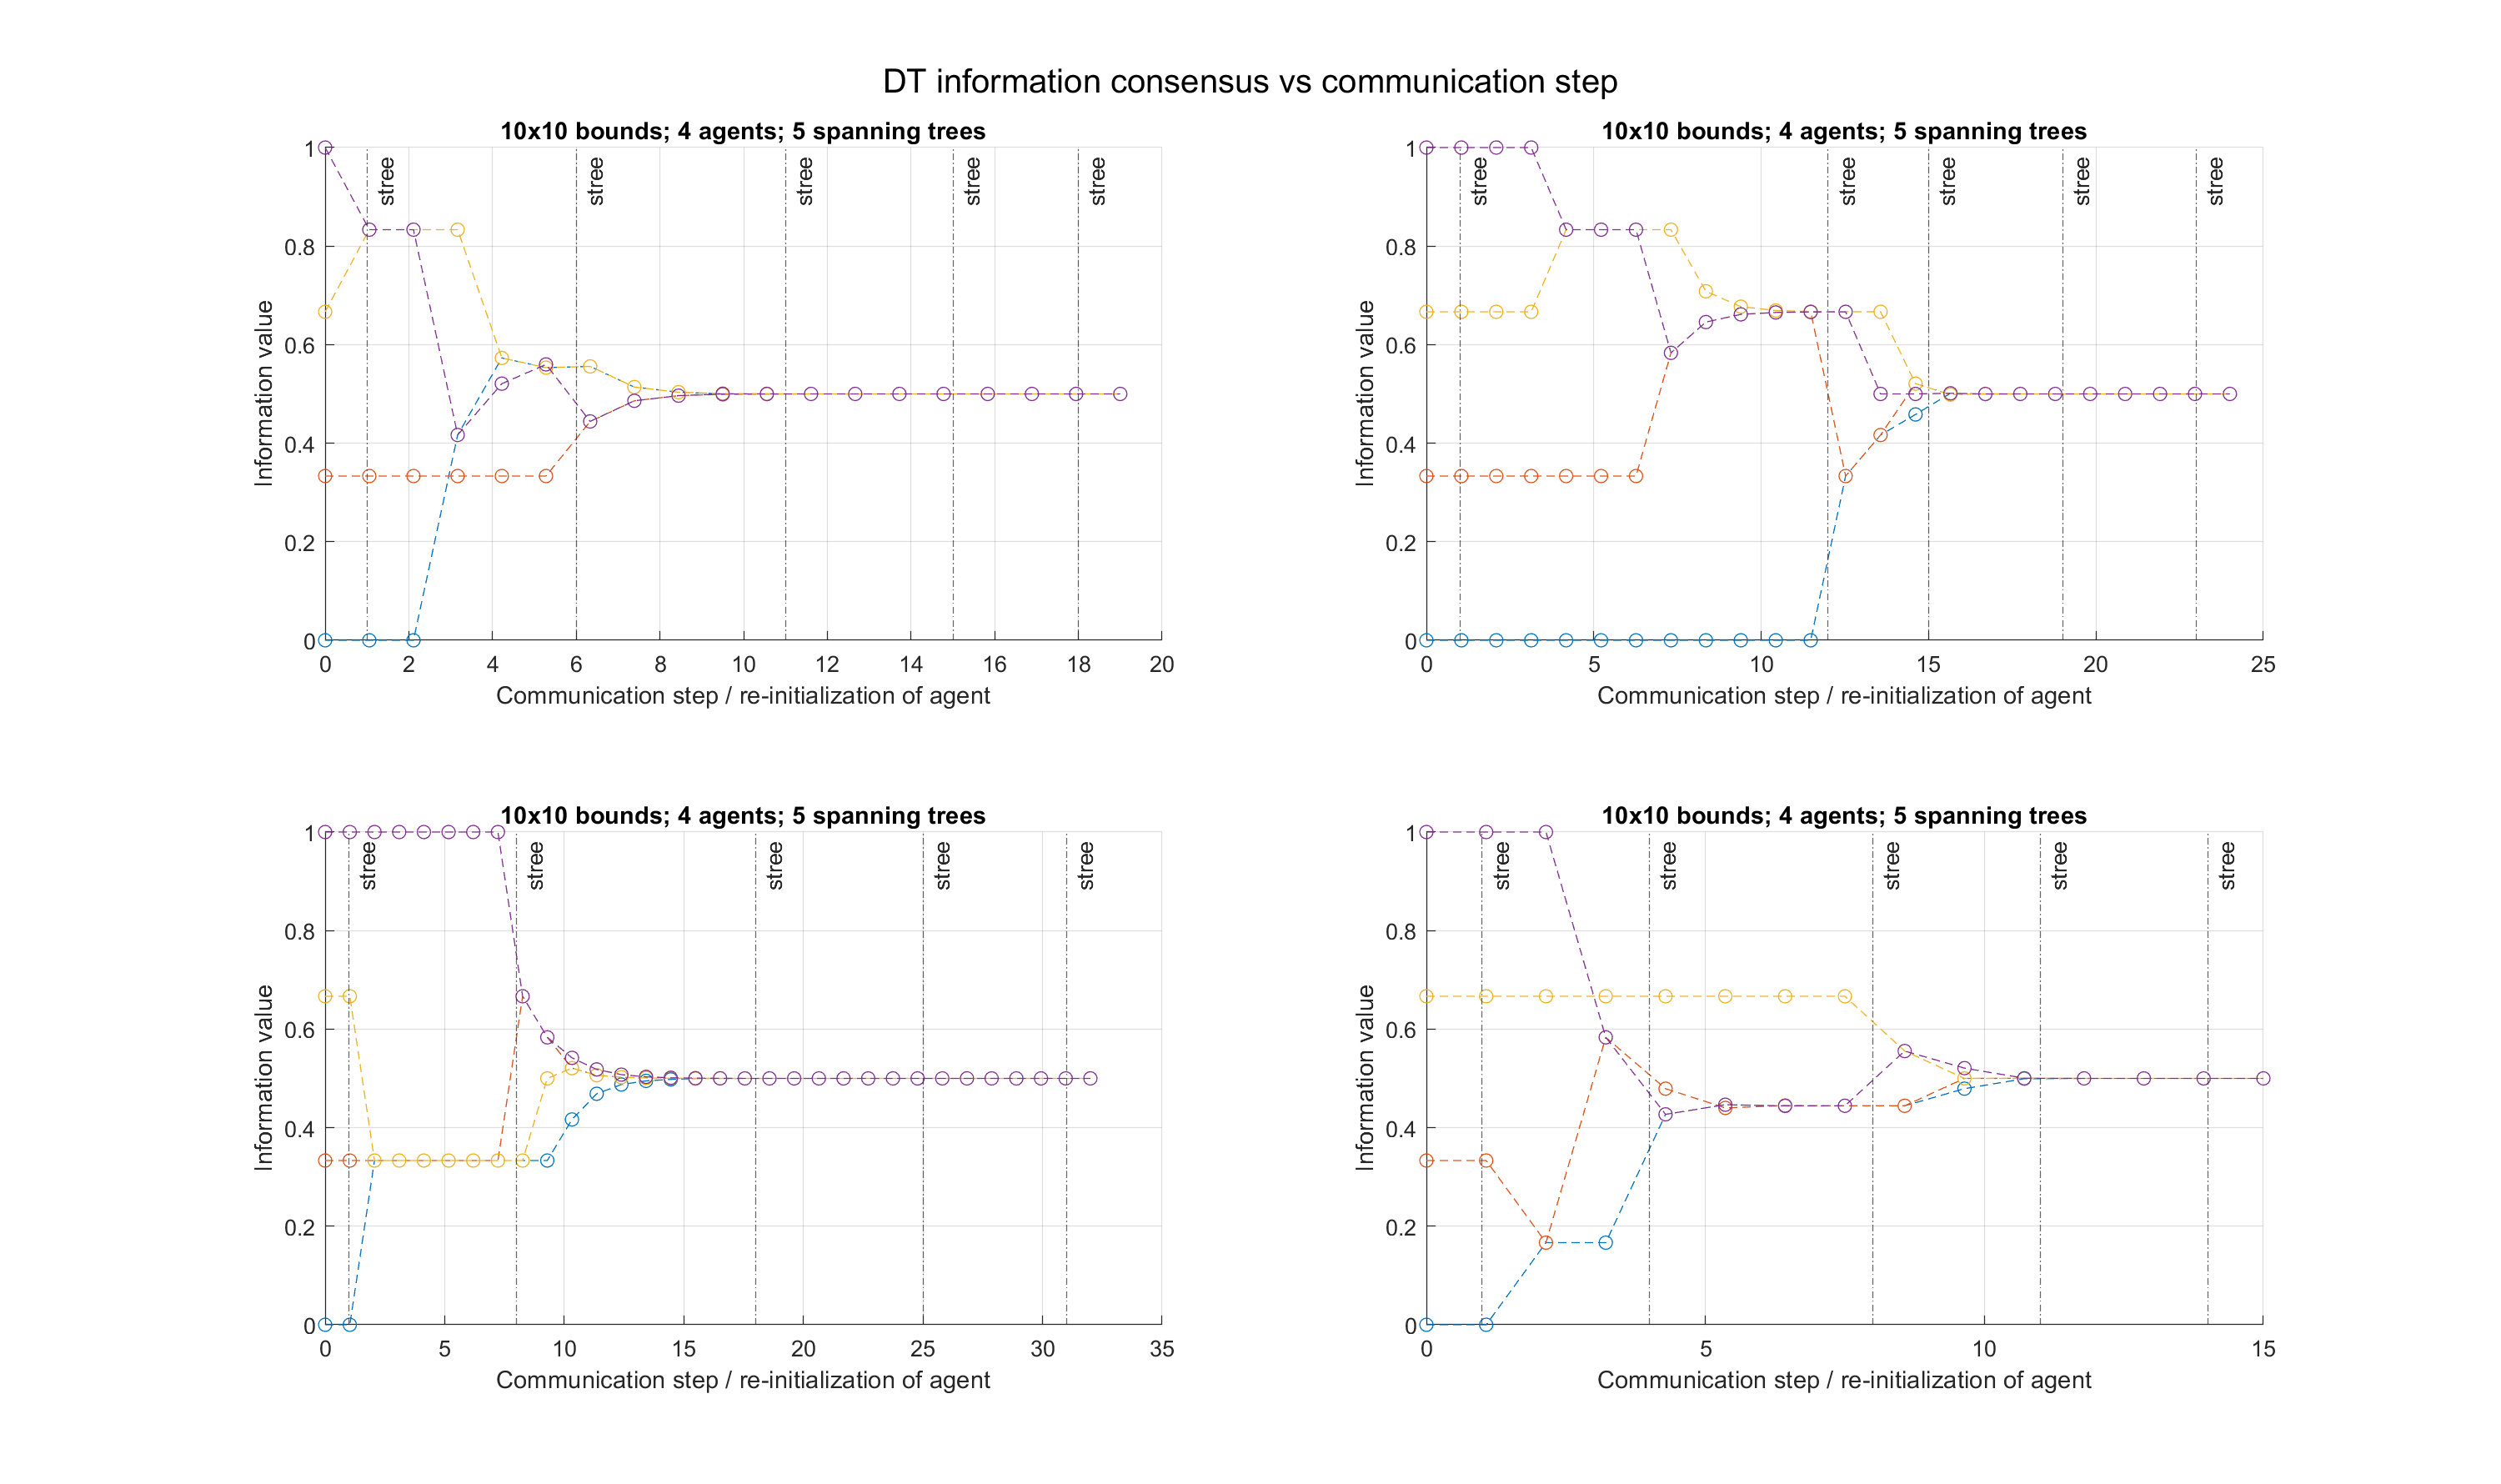
\includegraphics[width=\textwidth]{square10_4agent_5trees.png}
	\centering
\end{figure}

\begin{figure}[H]
	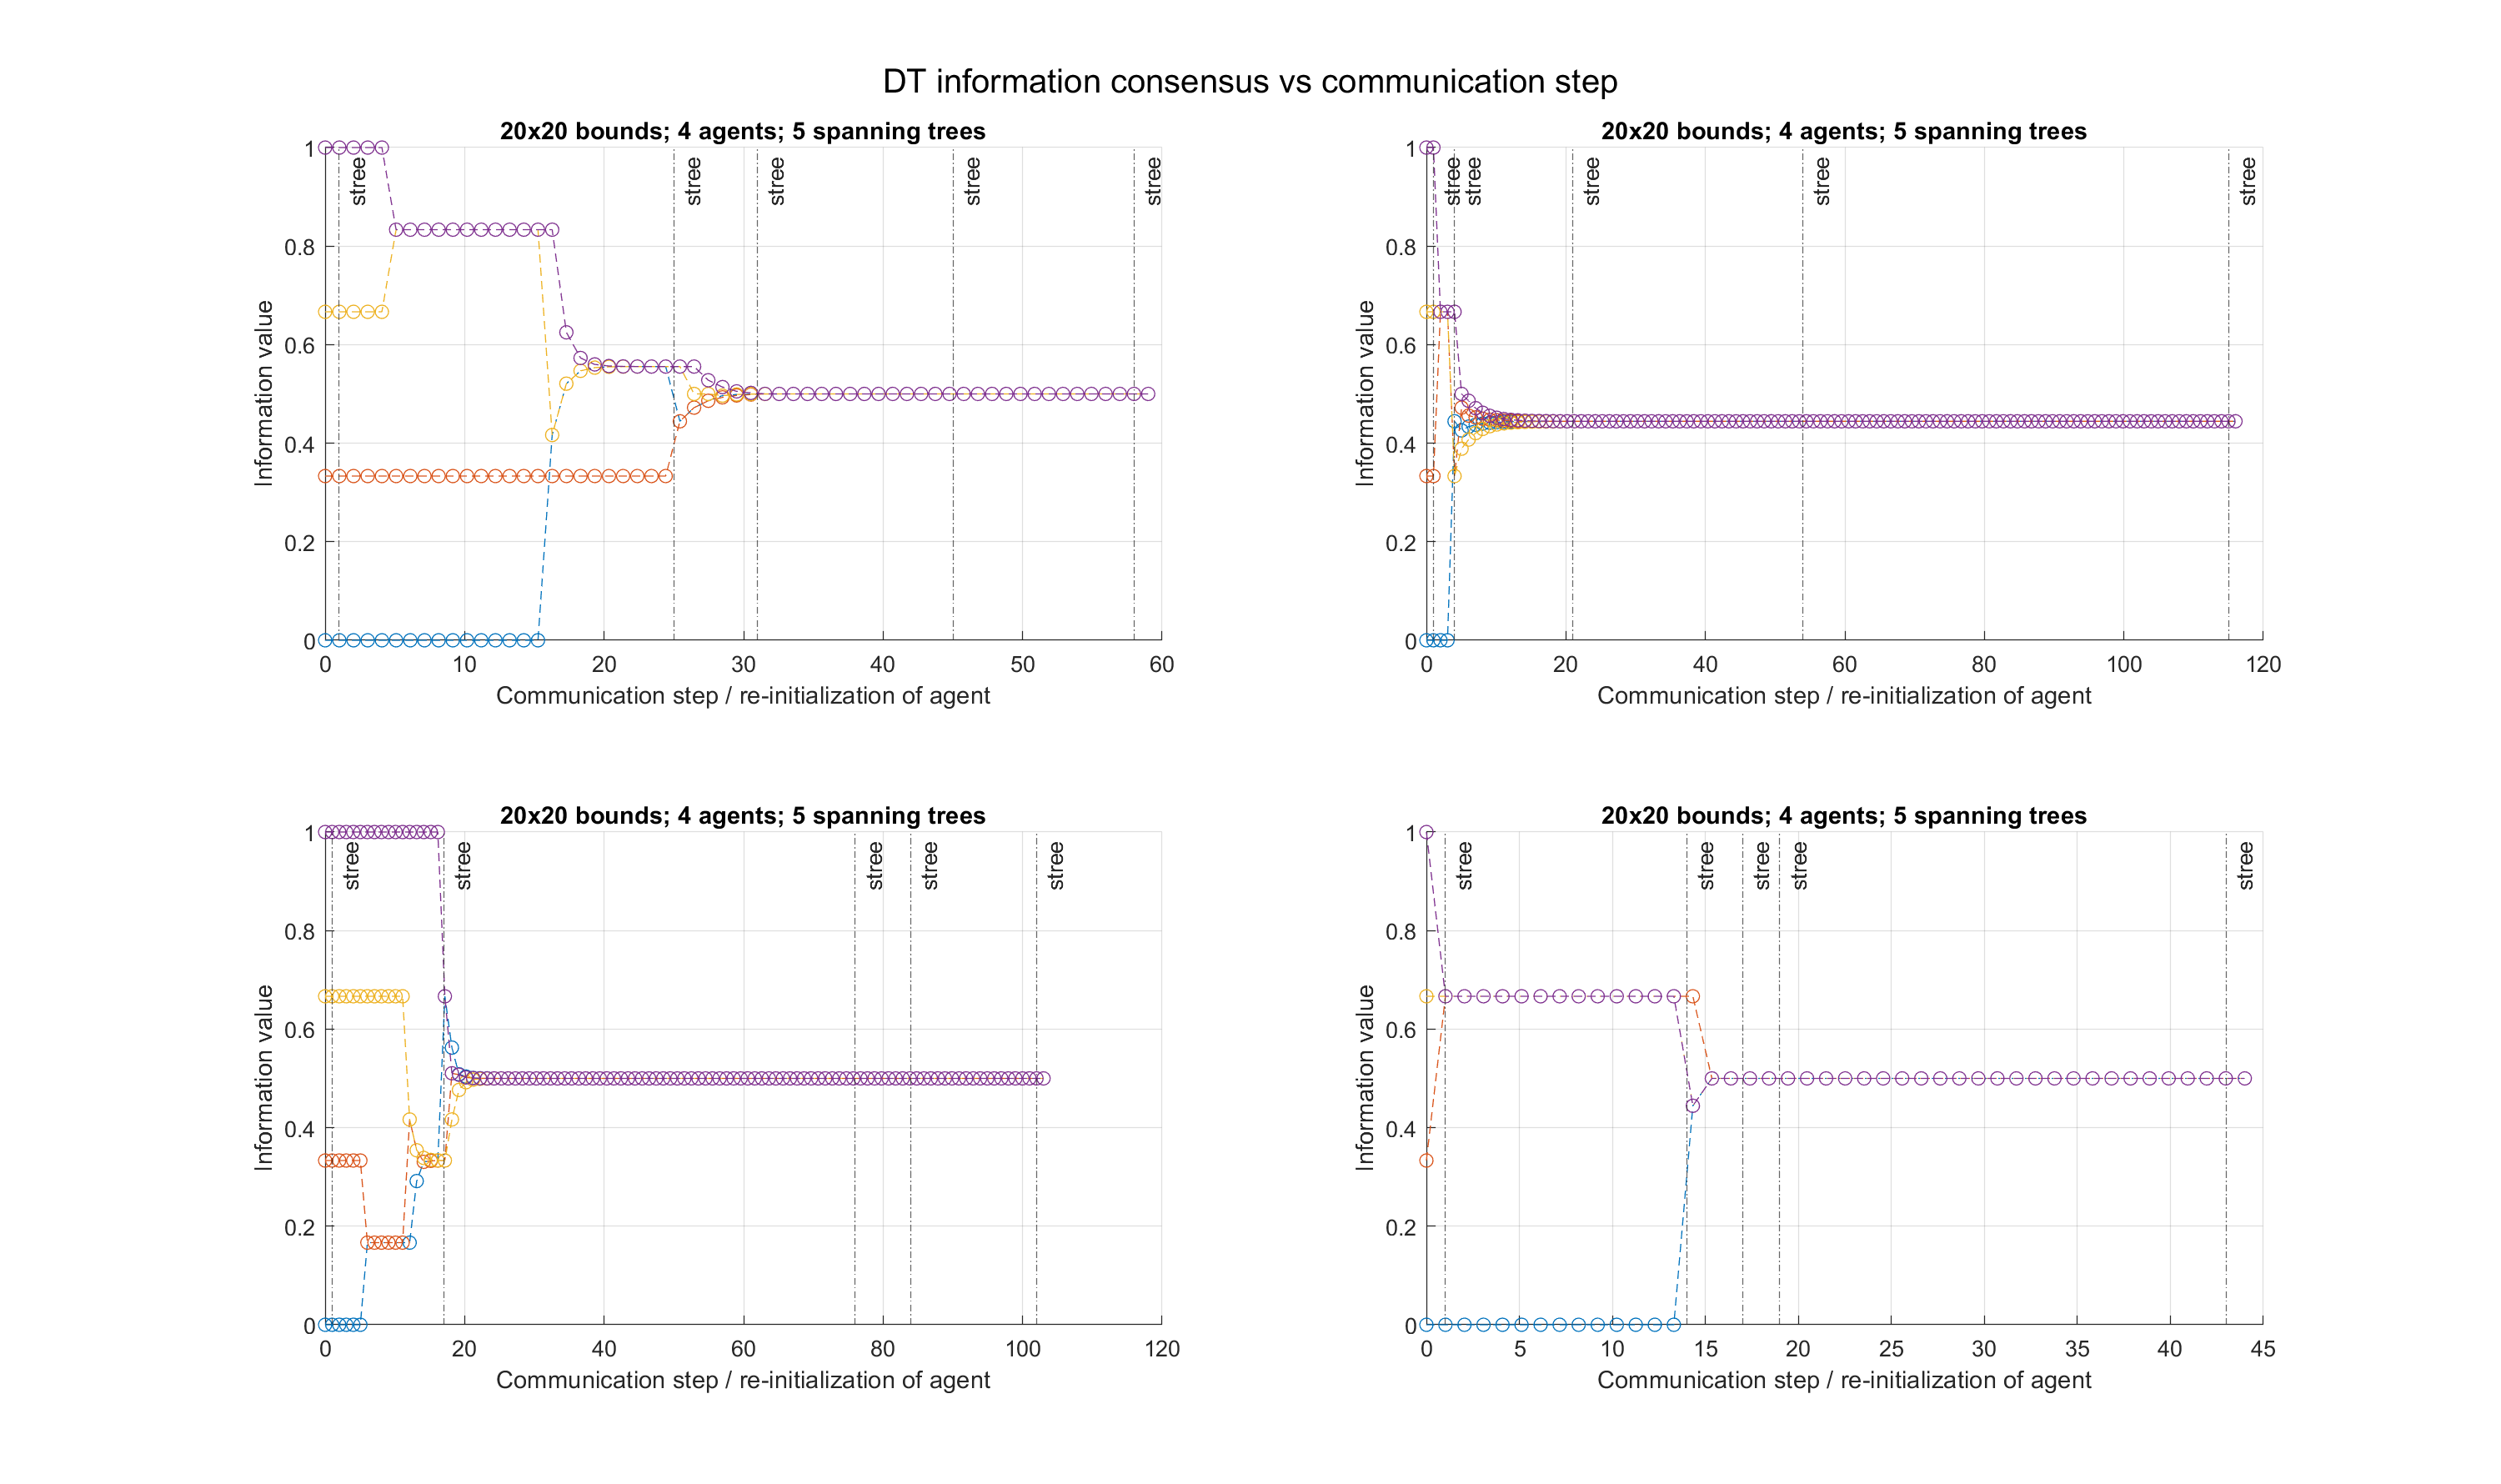
\includegraphics[width=\textwidth]{square20_4agent_5trees.png}
	\centering
\end{figure}

\begin{figure}[H]
	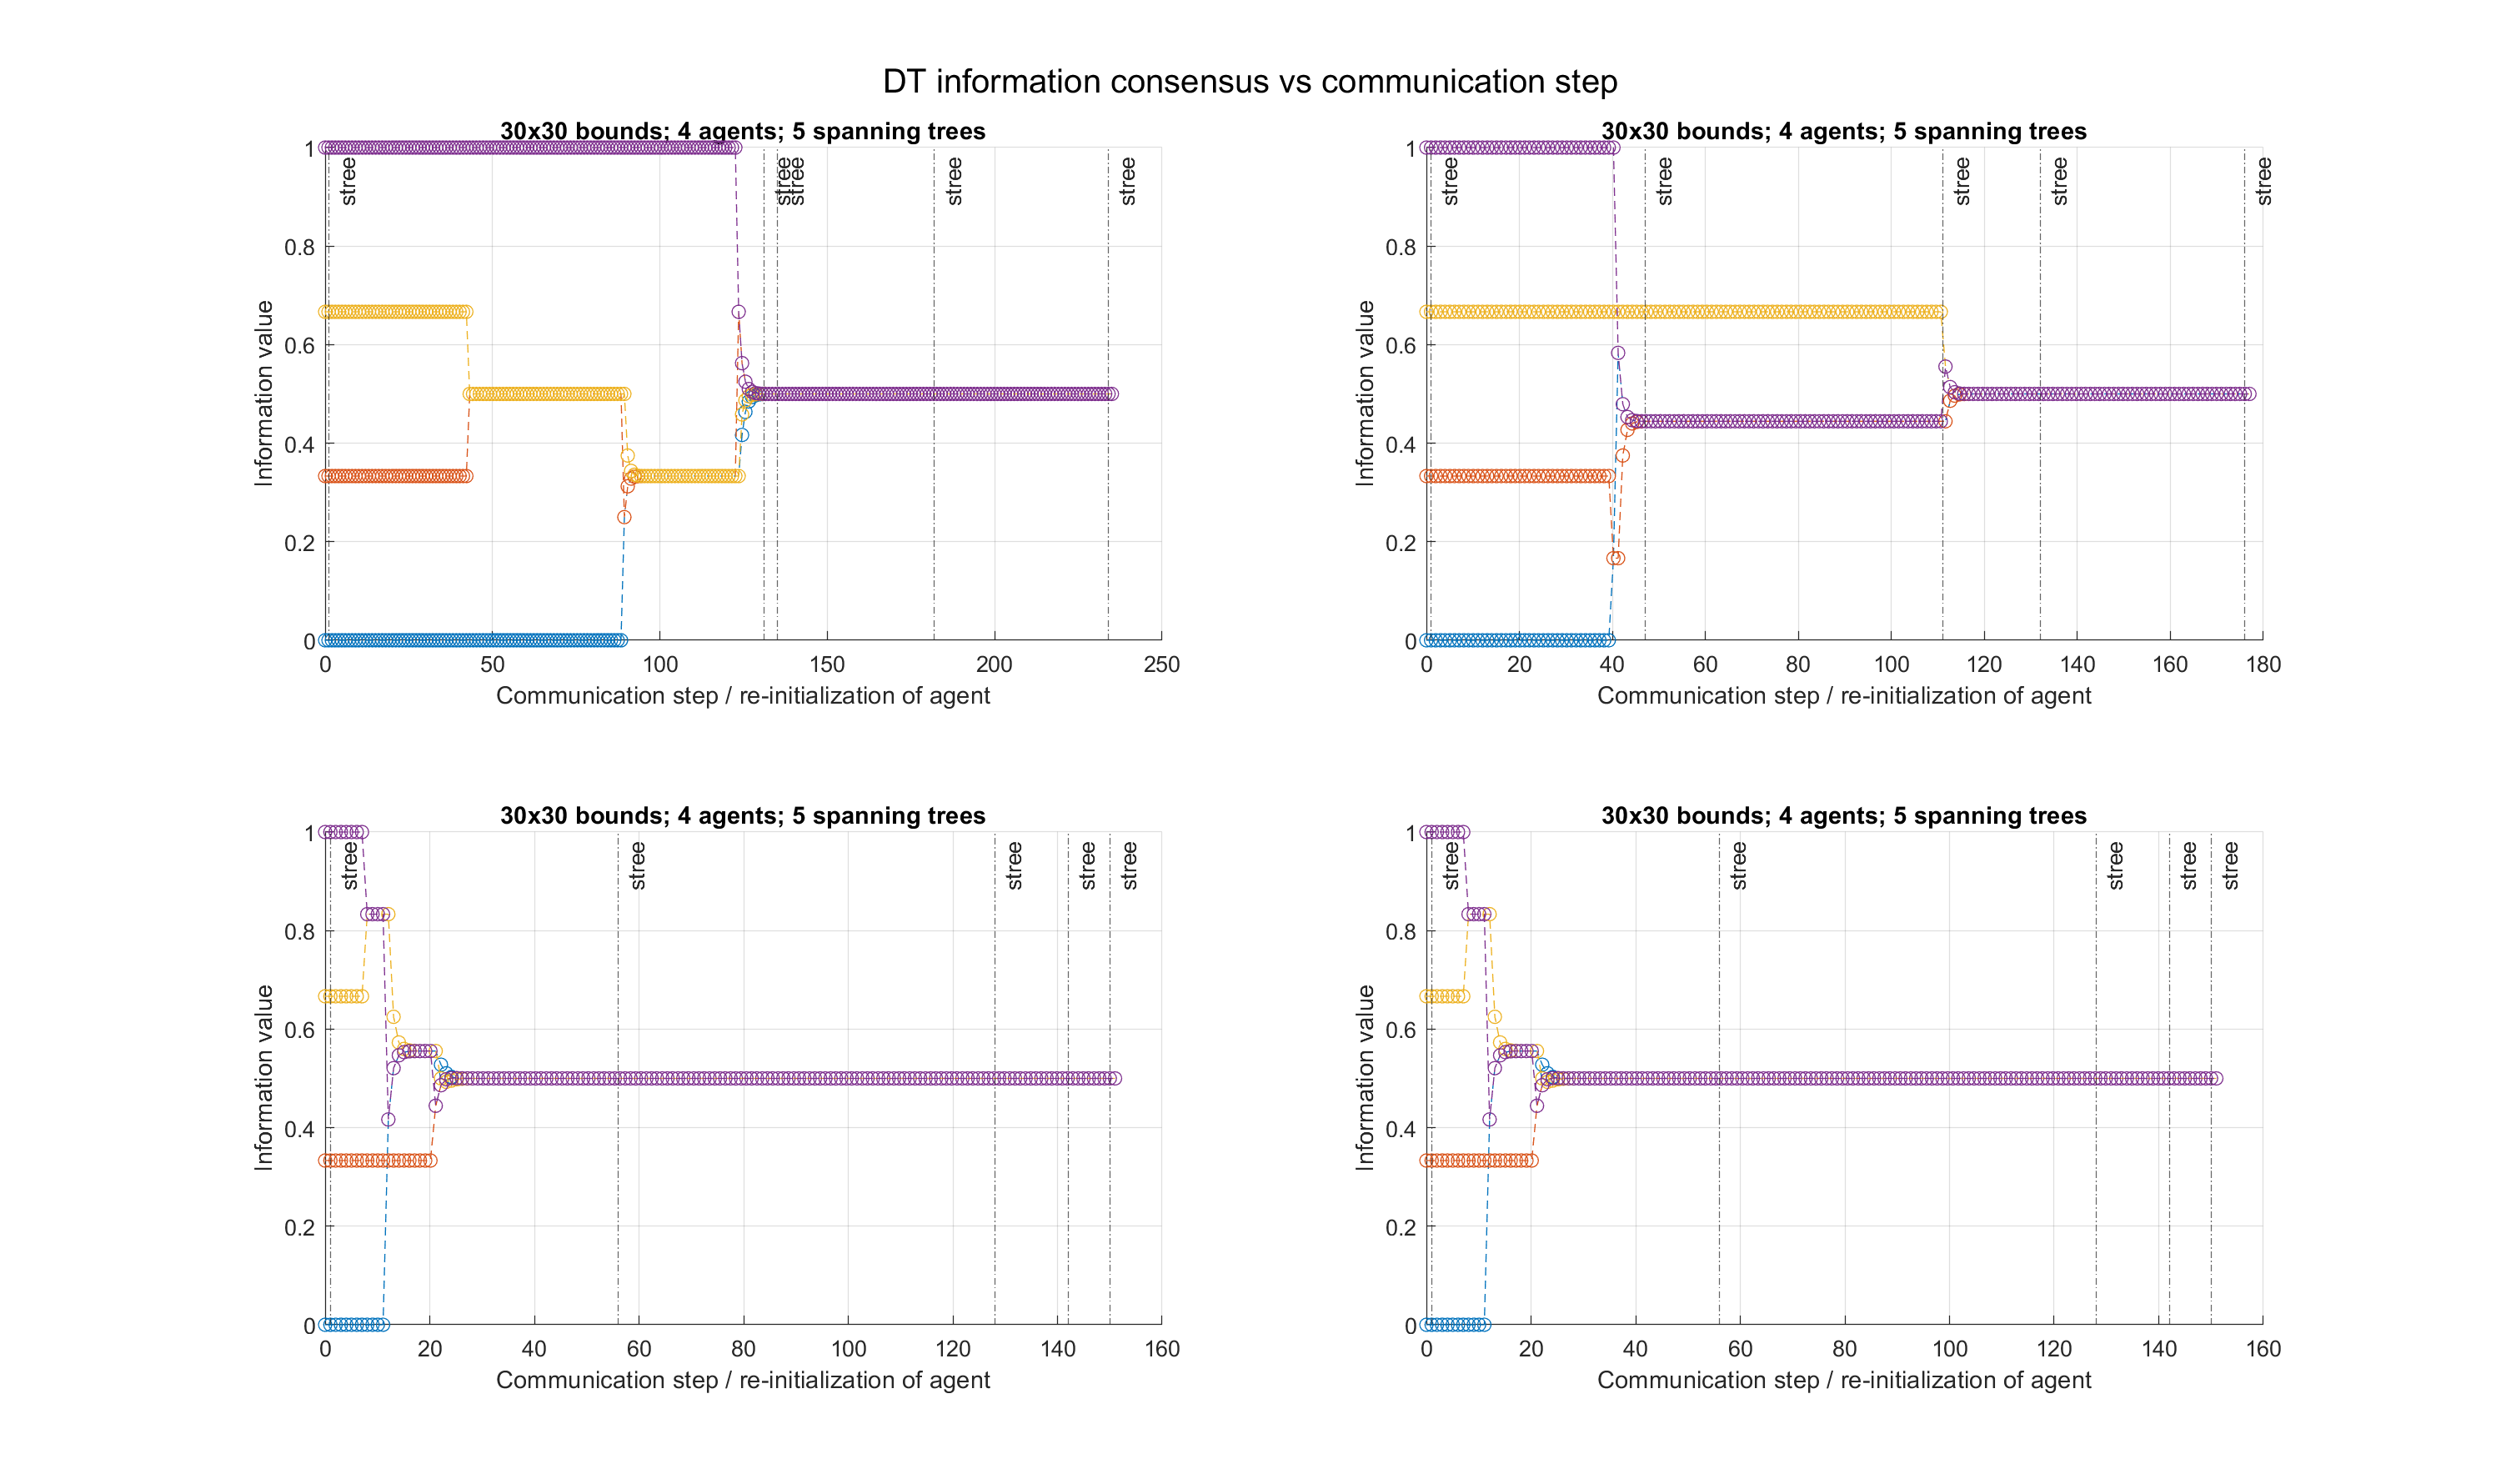
\includegraphics[width=\textwidth]{square30_4agent_5trees.png}
	\centering
\end{figure}

I've also included the distributions of steps required for the 1st and 3rd spanning trees to occur. Note that the formation of the modified $G$ made it easy for the 1st tree to be the trivial case, but this has no meaning when it comes to convergence.

\begin{figure}[H]
	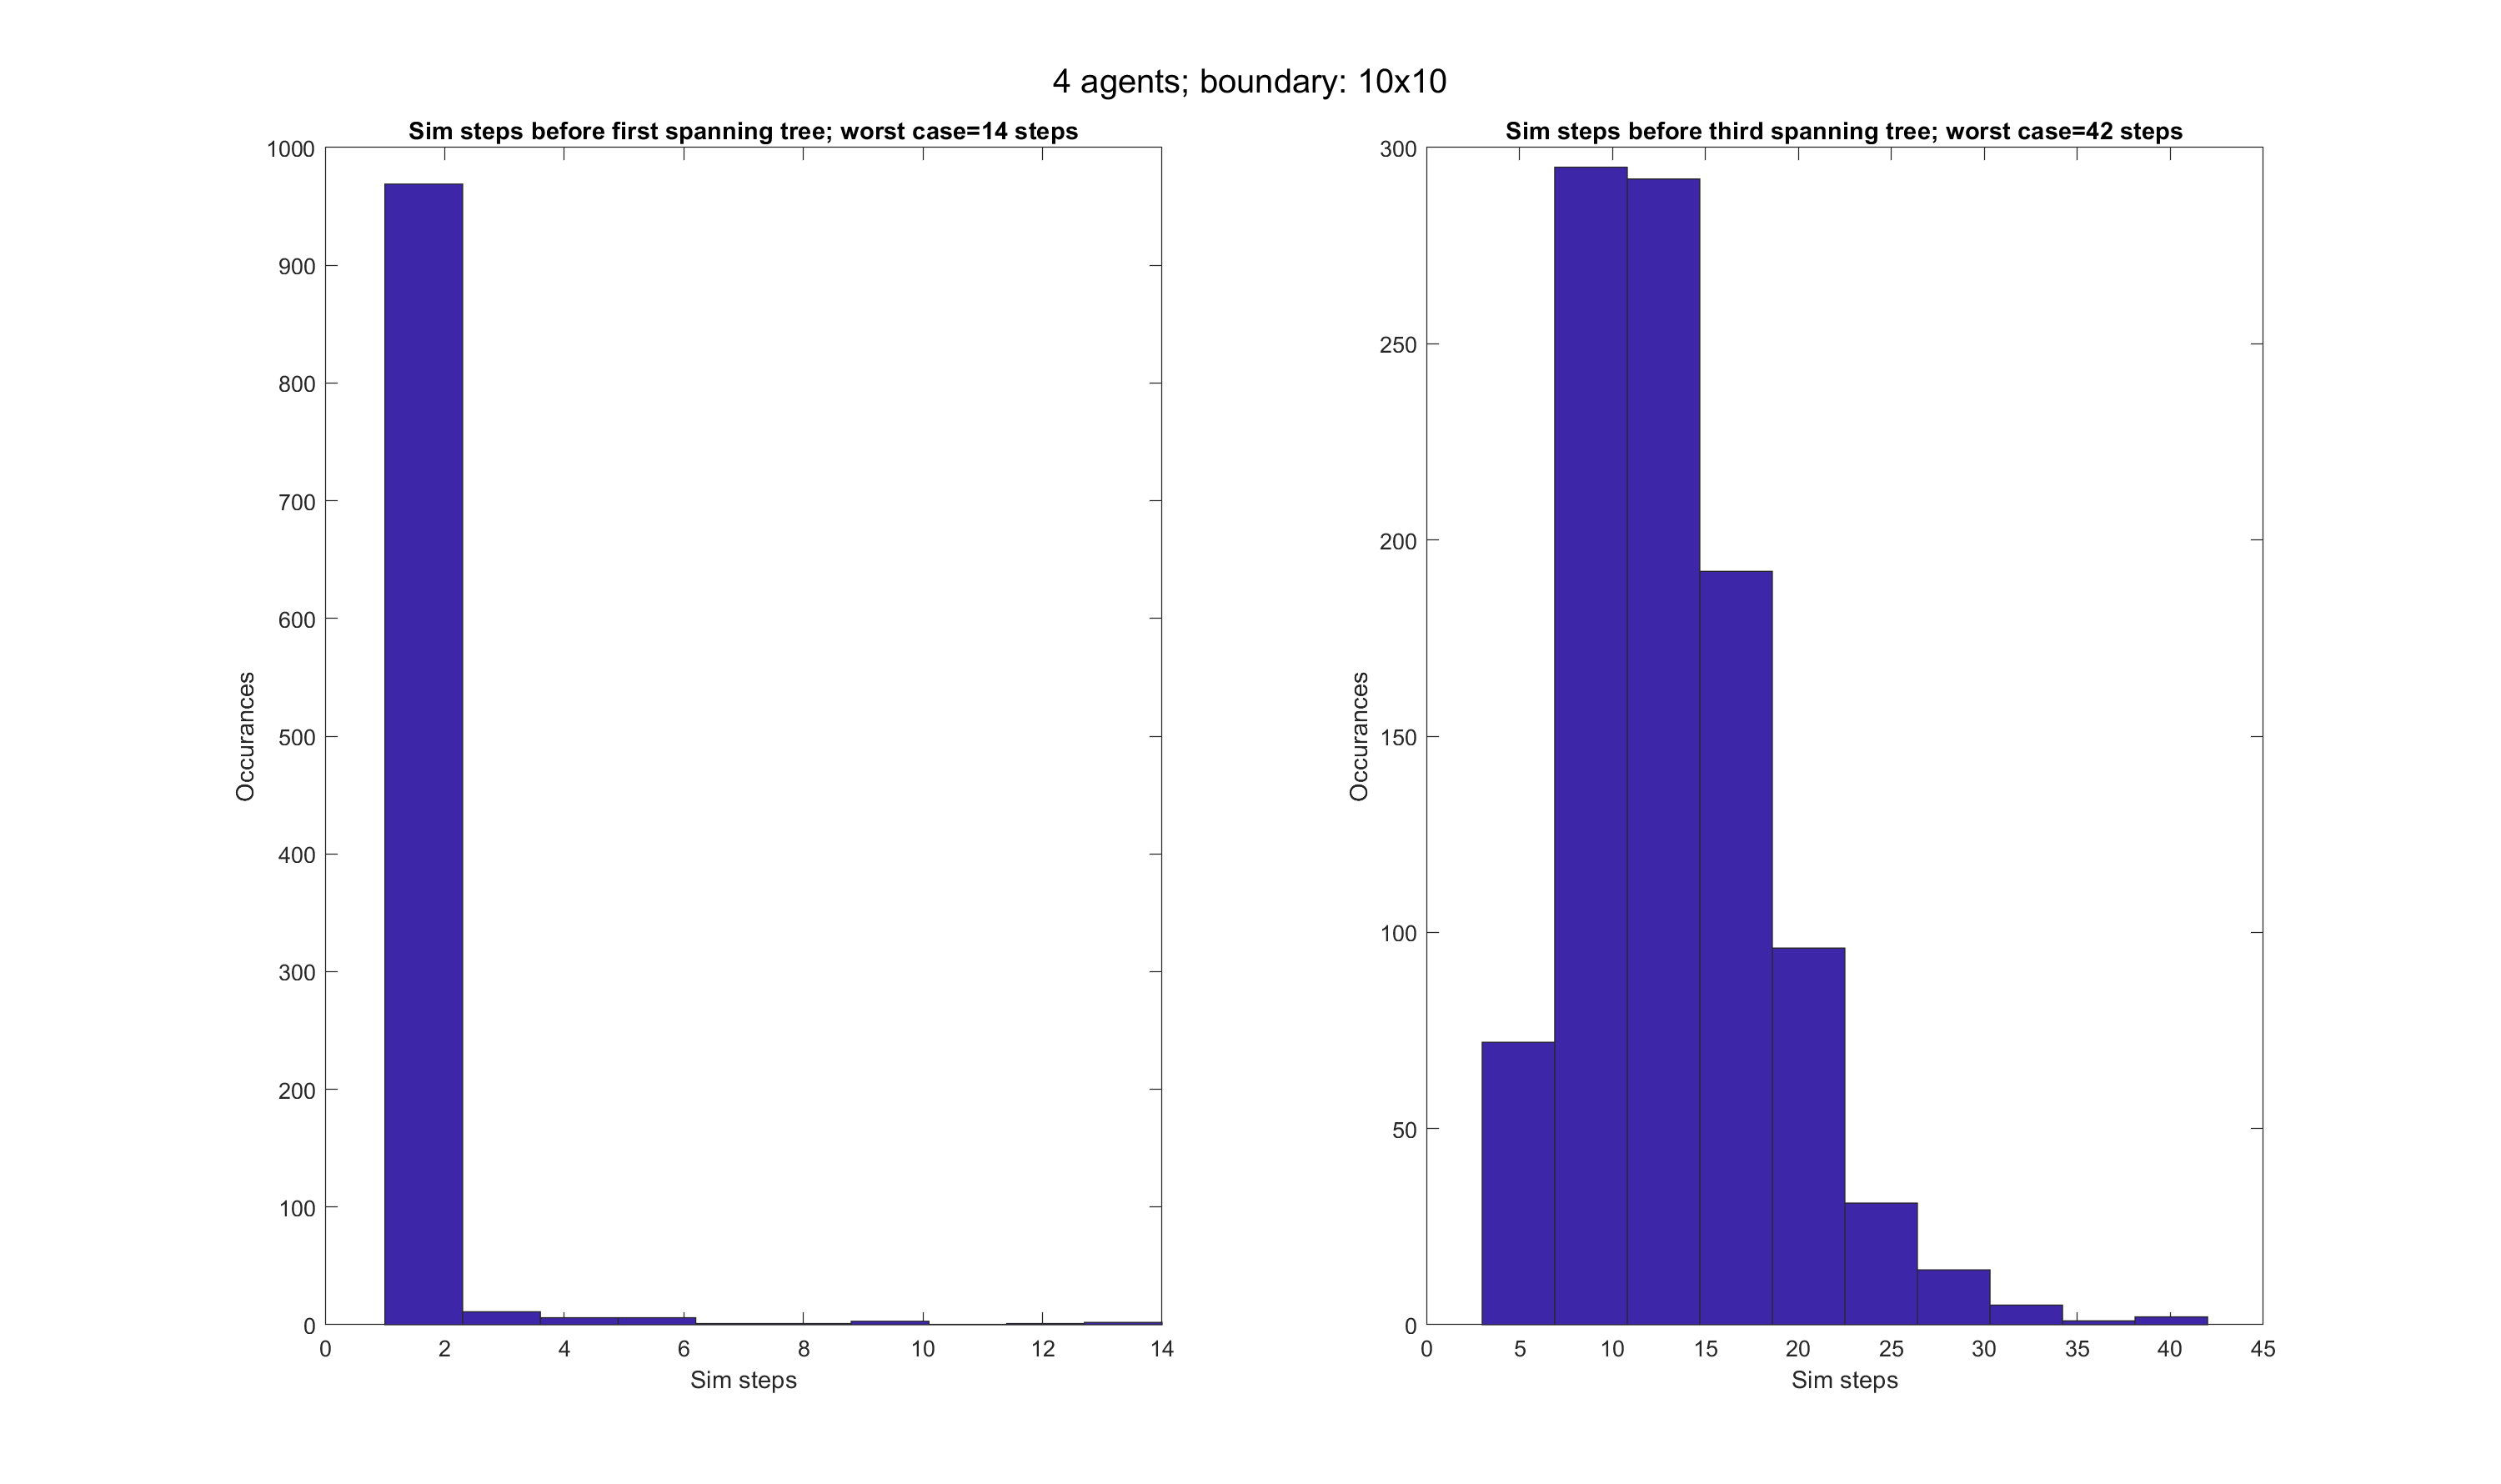
\includegraphics[width=\textwidth]{square10_4agent_5trees_stree_steps.png}
	\centering
\end{figure}

\begin{figure}[H]
	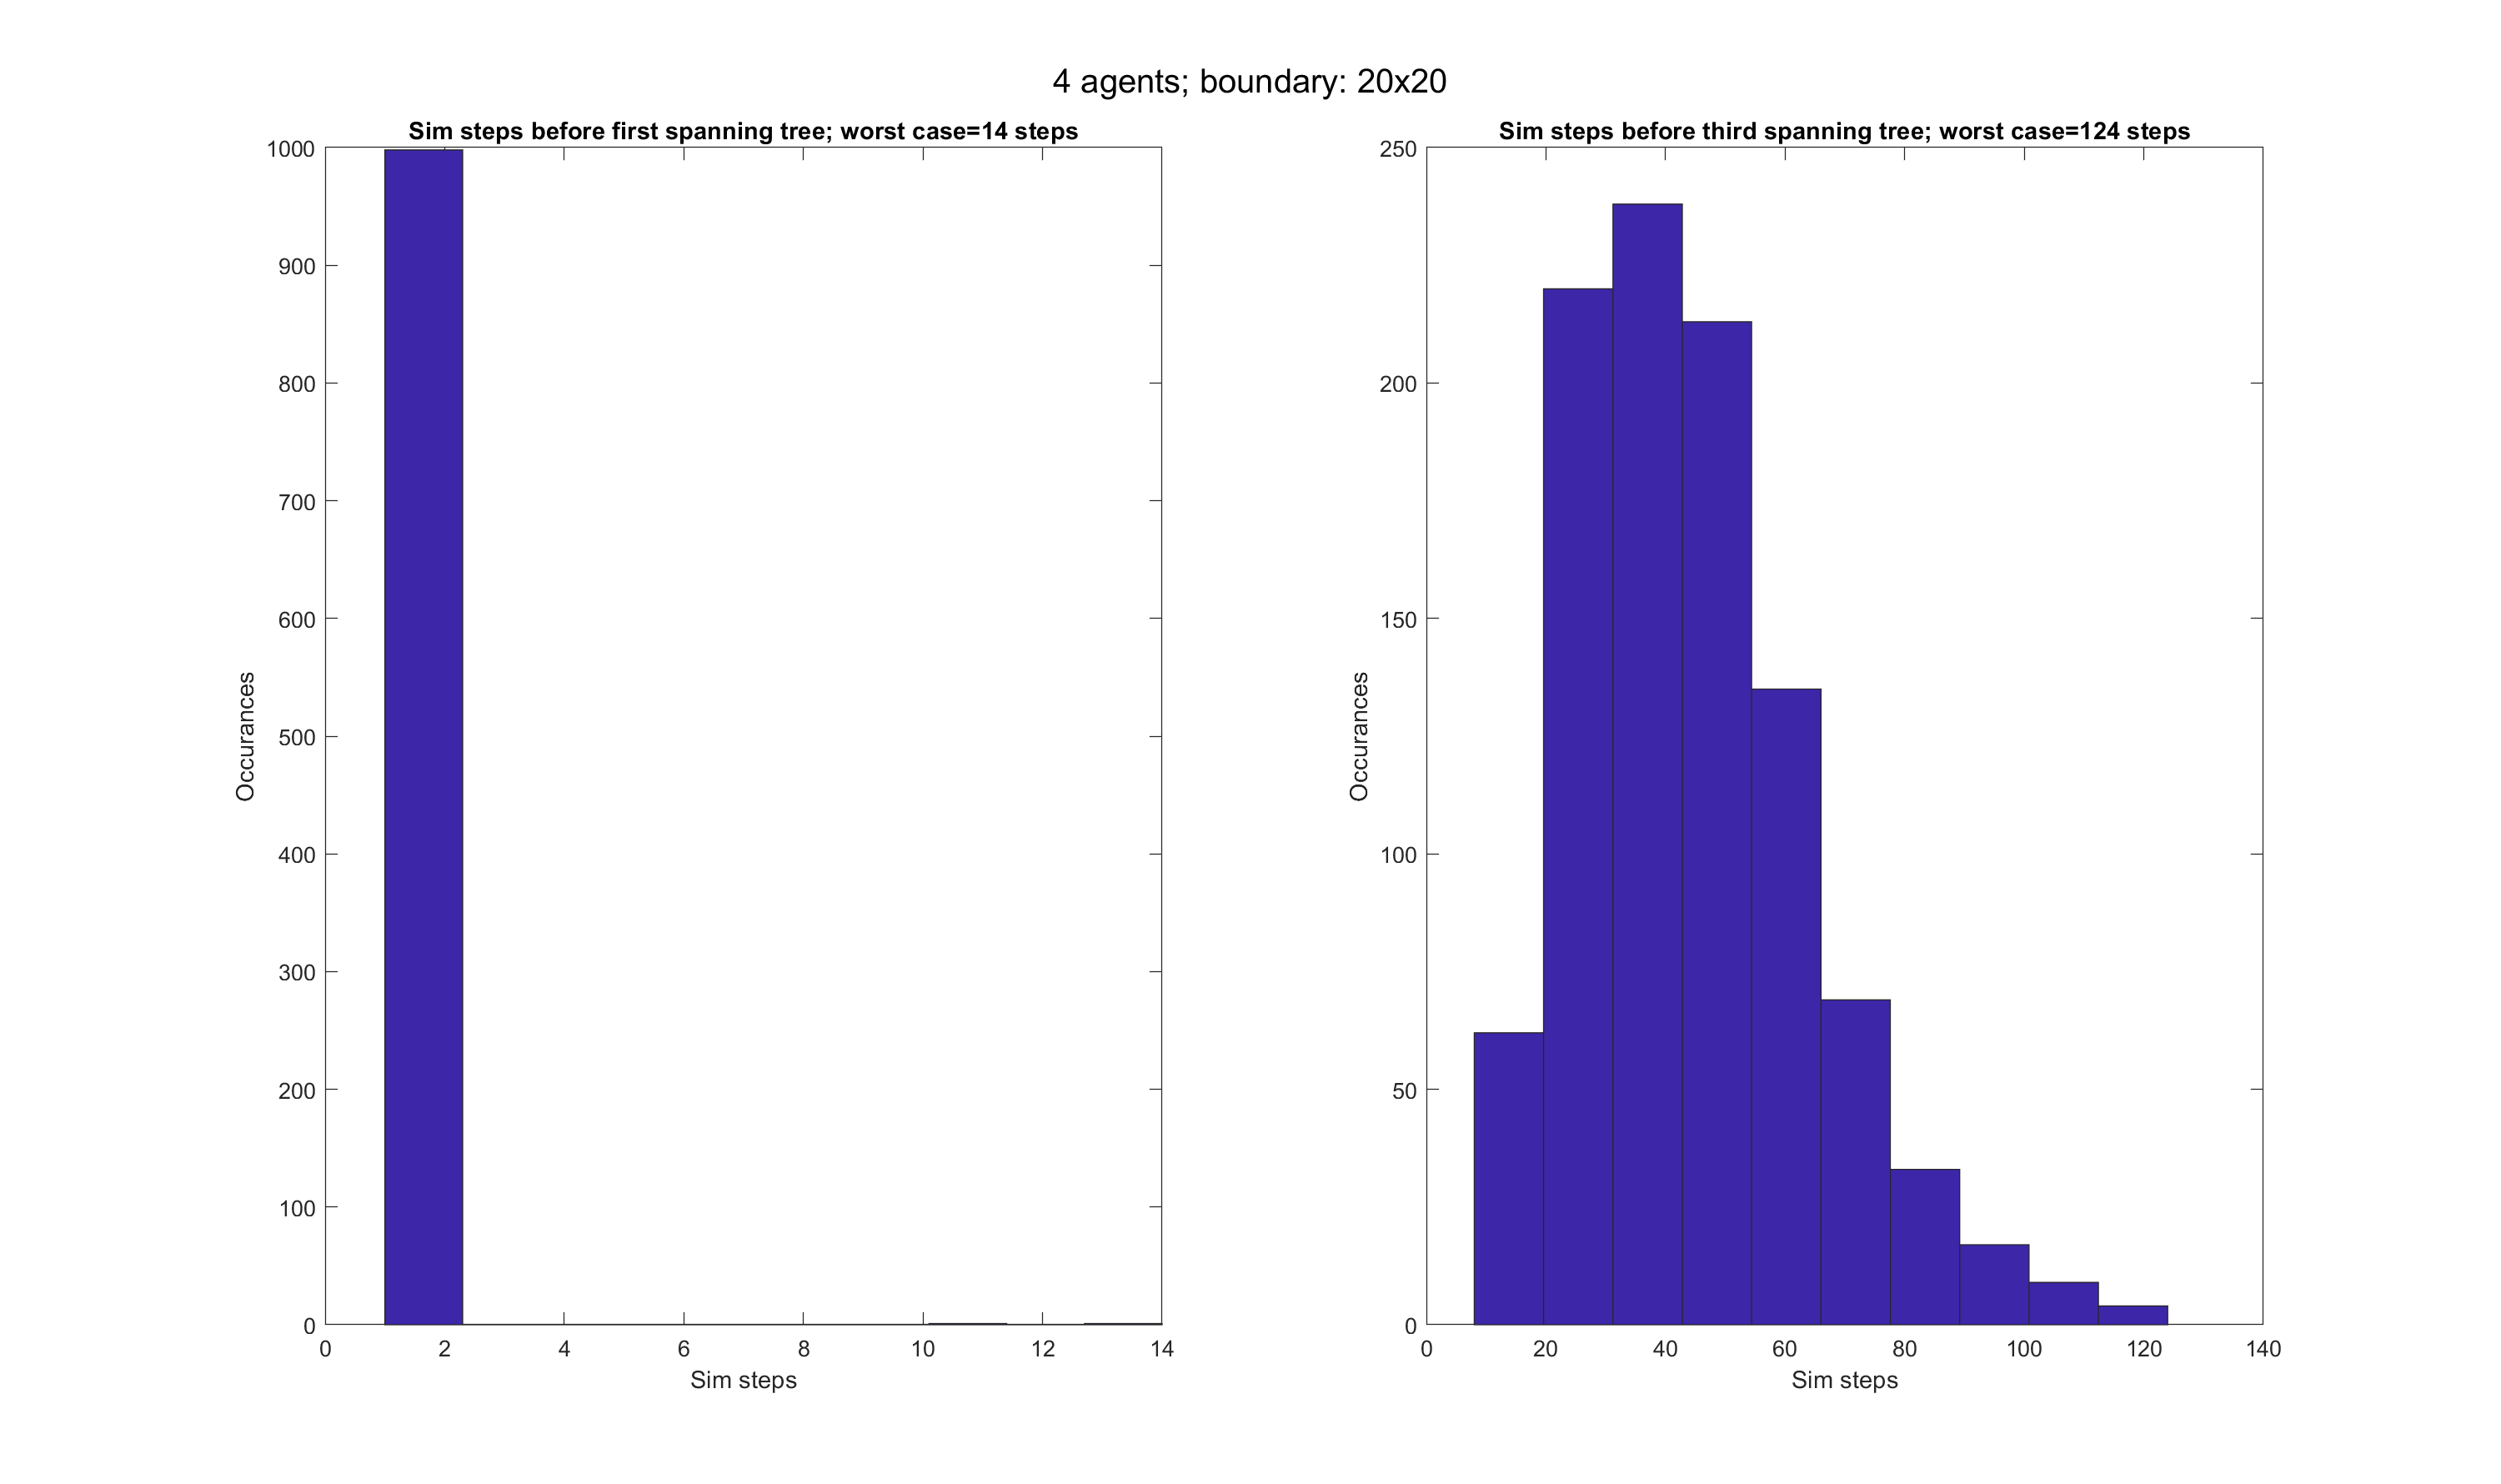
\includegraphics[width=\textwidth]{square20_4agent_5trees_stree_steps.png}
	\centering
\end{figure}

\begin{figure}[H]
	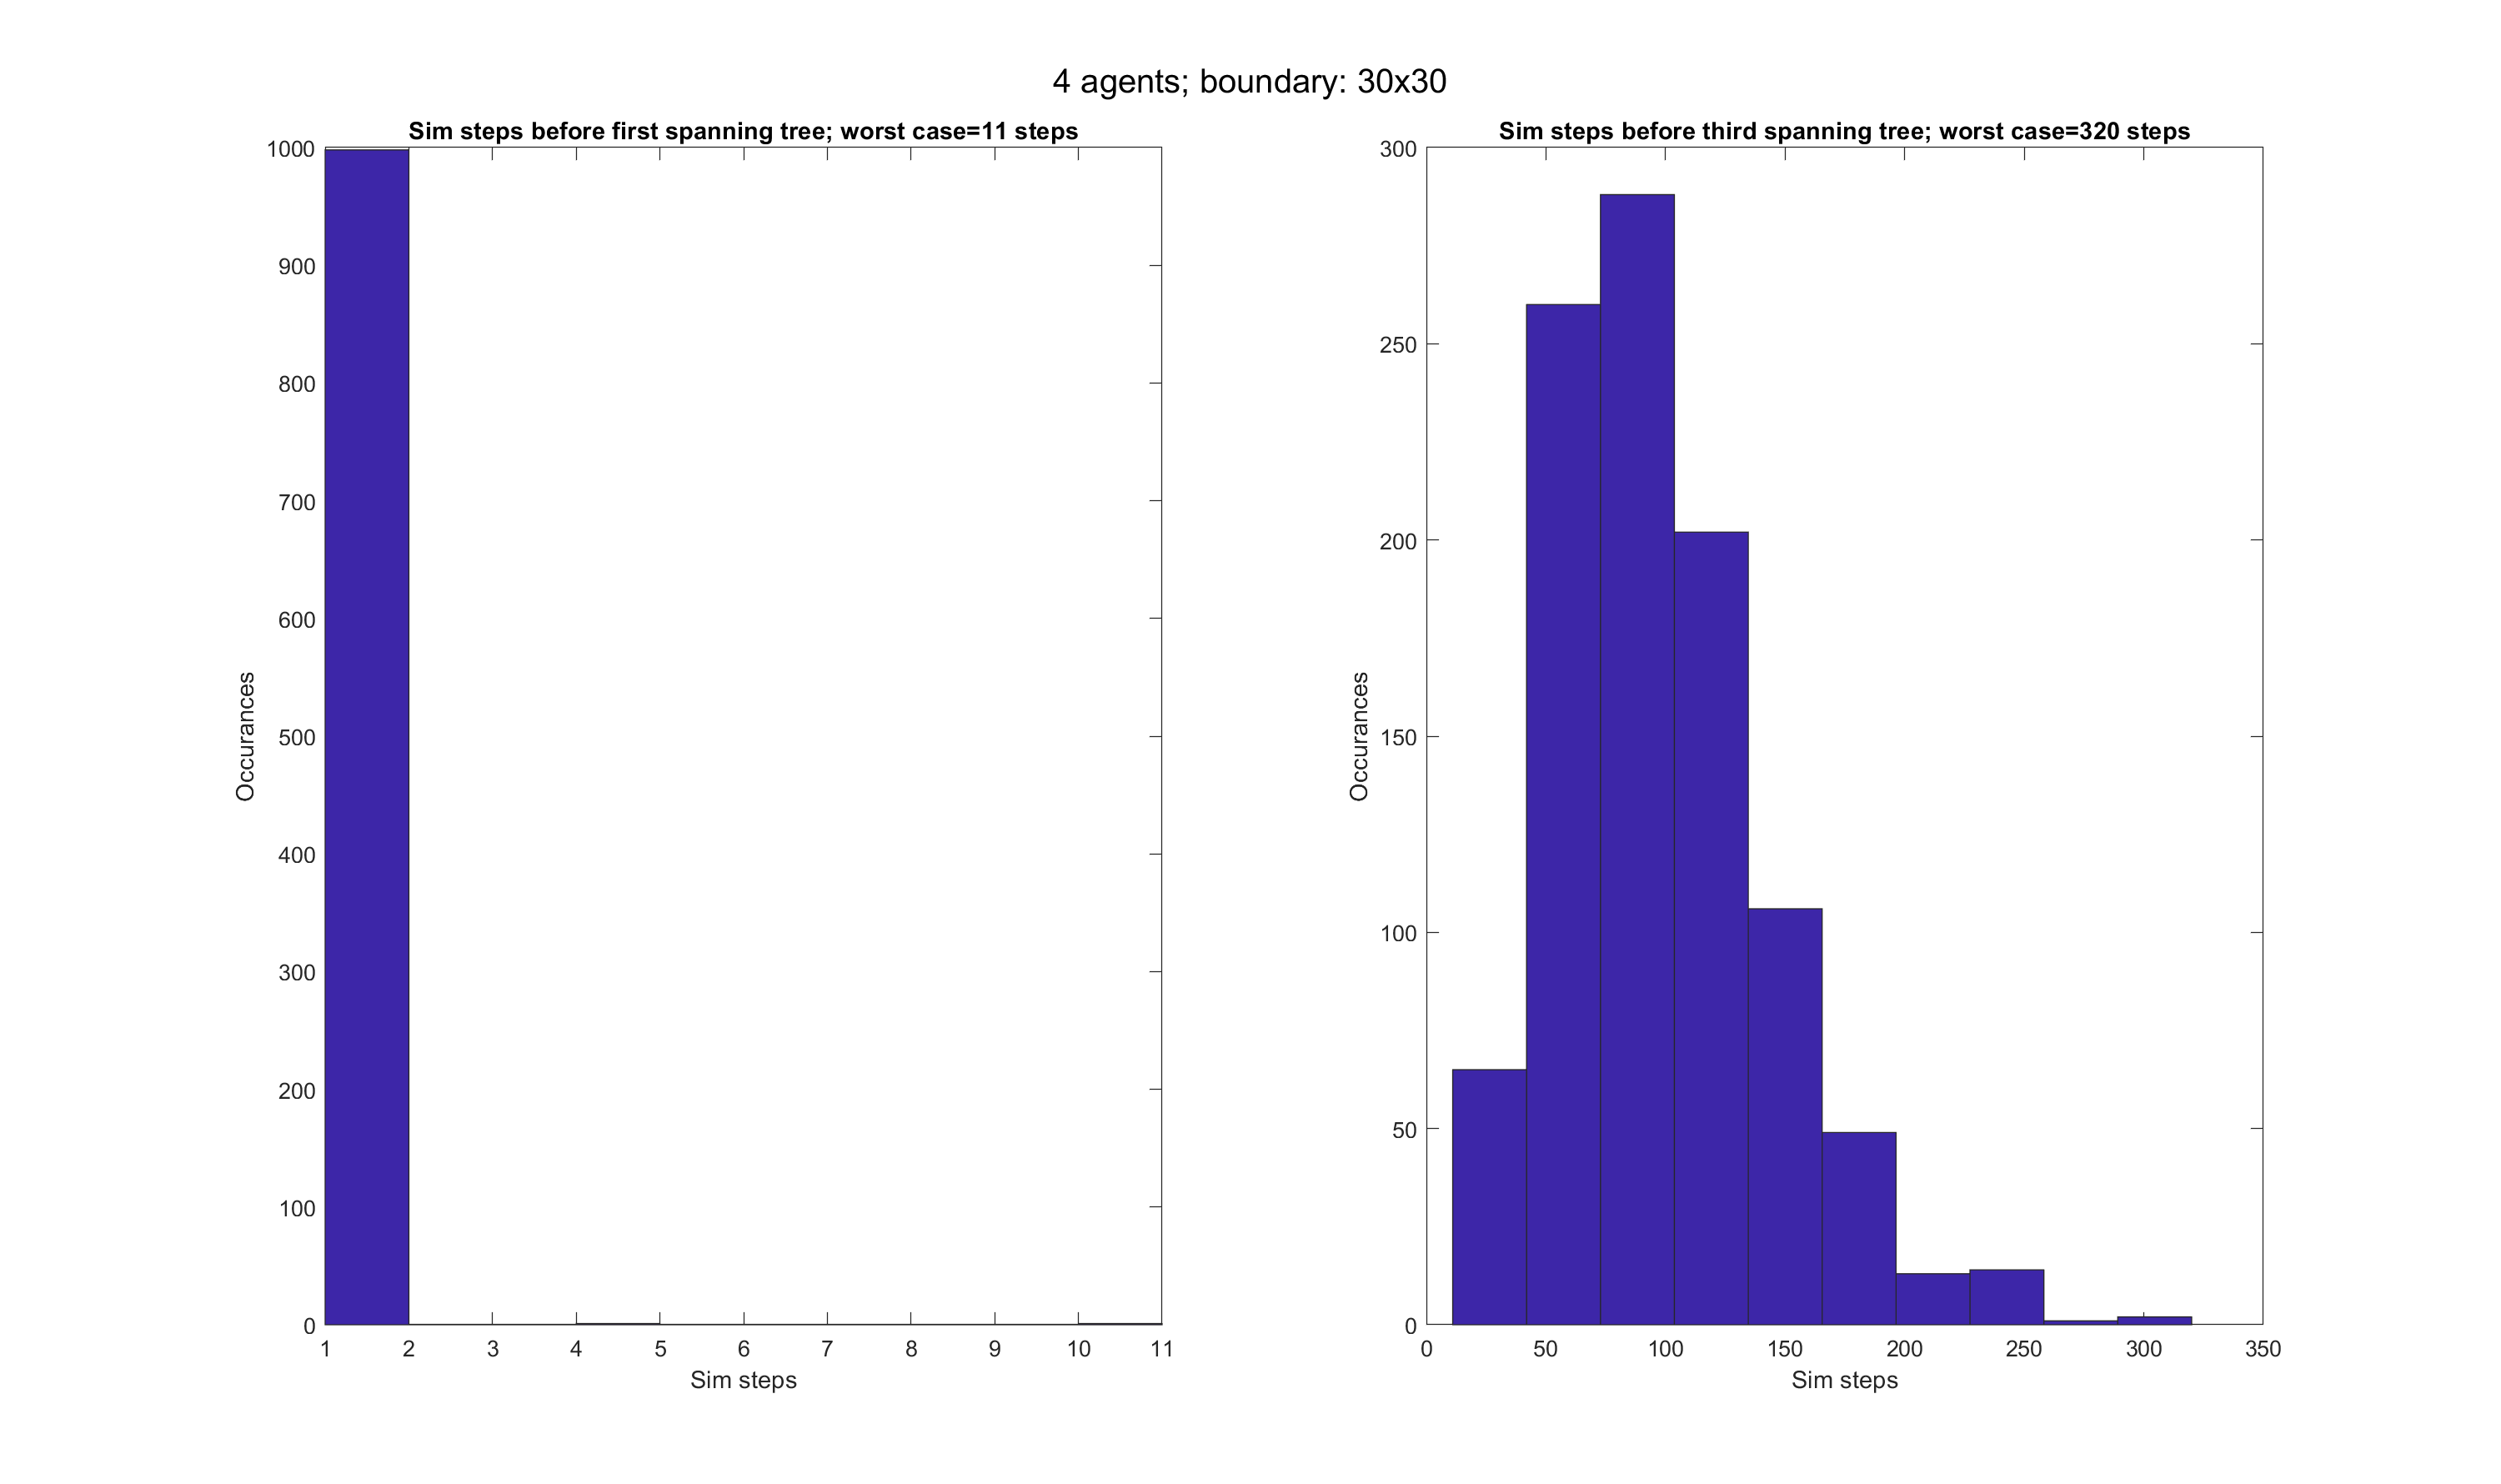
\includegraphics[width=\textwidth]{square30_4agent_5trees_stree_steps.png}
	\centering
\end{figure}

\section{Conclusions}\label{conclusions}
In short, I didn't know this technique existed to achieve consensus, but it's nice to confirm that it converges. Further analysis here could be to establish a safe threshold for the duration that buoyancy gliders need to be at sea before all information is shared successfully. We could also try the simulations for weighted directed matrices and see how that causes the convergence value to change. It is interesting to note that the convergence results here all appear to be average consensus, so that will need to be explained. We still need to determined how this would work for discrete message passing (secret key), because here we rely on dynamic updates to the agent's information. A really nice thing to note is that this result is not time-dependent, the formulation here is decoupled from time and only relies on communication updates (event-driven). Lastly, I would like to compare and contrast this approach to more strictly algebraic graph theory based approaches, eg: no stochastic element. We should also look at how the information converges for more agents, as it seems the agents converge in pairs, eg: 16x1 -> 8x2 -> 4x4 -> 2x8 -> 1x16 (converged). Also, how robust is this convergence to noise in the information or position solution? \\

[1] "Consensus of Information Under Dynamically Changing Interaction Topologies" by W. Ren

\bibliographystyle{abbrv}
\bibliography{main}

\end{document}
